% 97-47(97쪽) — $B=C=30^\circ$ 인 이등변삼각형 ABC 와 그 외접원(원문 「오른쪽 그림」 · 지름 12 가 점 C 에서 끝난다). 스캔 화질이 낮아 TikZ 로 다시 그림.
% 라벨은 원문 것만: 꼭짓점 A·B·C, 두 각의 $30^\circ$, 지름의 $12$. 삼각형의 넓이(답)가 읽히지 않게 변의 길이는 적지 않는다.
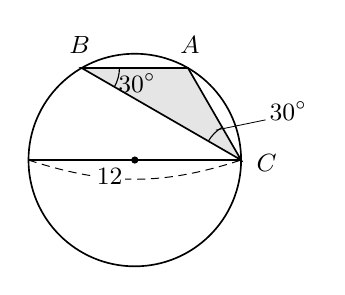
\begin{tikzpicture}[line width=0.6pt, x=1cm, y=1cm]
  \coordinate (A) at (0.675,1.169);
  \coordinate (B) at (-0.675,1.169);
  \coordinate (C) at (1.35,0);
  \fill[black!10] (A) -- (B) -- (C) -- cycle;
  \draw (0,0) circle (1.35);
  \draw (A) -- (B) -- (C) -- cycle;
  % 지름
  \draw[line width=0.45pt] (-1.35,0) -- (1.35,0);
  \fill (0,0) circle (1.3pt);
  \draw[densely dashed, line width=0.35pt] (-1.35,0) to[bend right=18] (1.35,0);
  \node[font=\small, fill=white, inner sep=1pt] at (-0.32,-0.205) {$12$};
  % 두 각의 표시
  \draw[line width=0.4pt] ([shift=(-30:0.48)]B) arc (-30:0:0.48);
  \node[font=\small] at (0.030,0.980) {$30^\circ$};
  \draw[line width=0.4pt] ([shift=(120:0.48)]C) arc (120:150:0.48);
  \node[font=\small] at (1.95,0.62) {$30^\circ$};
  \draw[line width=0.3pt] (1.66,0.51) -- (1.03,0.38);
  \node[font=\small, anchor=south] at (0.70,1.22) {$\pt{A}$};
  \node[font=\small, anchor=south] at (-0.70,1.22) {$\pt{B}$};
  \node[font=\small, anchor=west] at (1.42,-0.04) {$\pt{C}$};
\end{tikzpicture}
